\documentclass[12pt,letterpaper,twoside]{article}
\usepackage{cme211}
\usepackage{algorithm2e}

\def\D{\mathrm{d}}
\usepackage{atbegshi}% http://ctan.org/pkg/atbegshi
\AtBeginDocument{\AtBeginShipoutNext{\AtBeginShipoutDiscard}}

\begin{document}
\title{Lecture 12: File IO in C++\vspace{-5ex}}
\date{November 3rd, 2018}
\maketitle

{\footnotesize
\paragraph{Topics Introduced:} Command line arguments, string
formatting, File IO, functions, the pre-processor and \texttt{\#include}.
}
\vspace{-3ex}

\subsection{Command line arguments}
\begin{cpp}
#include <iostream>

int main(int argc, char *argv[]) {
  // Display the command line arguments
  for (int n = 0; n < argc; n++) {
    std::cout << n << " " << argv[n] << std::endl;
  }
  return 0;
}
\end{cpp}

Output:

\begin{verbatim}
$ ./argv1 hello.txt 3.14 42
0 ./argv1
1 hello.txt
2 3.14
3 42
\end{verbatim}

\subsubsection{Command line arguments}
\begin{cpp}
#include <iostream>
#include <string>

int main(int argc, char *argv[]) {
  if (argc < 4) {
    std::cout << "Usage:" << std::endl;
    std::cout << " " << argv[0] << " <filename> <param1> <param2>" << std::endl;
    return 0;
  }

  std::string filename = argv[1];
  double param1 = std::stof(argv[2]);
  int param2 = std::stoi(argv[3]);

  std::cout << "filename = " << filename << std::endl;
  std::cout << "param1 = " << param1 << std::endl;
  std::cout << "param2 = " << param2 << std::endl;

  return 0;
}
\end{cpp}

Output:

\begin{verbatim}
$ g++ -std=c++11 -Wall -Wconversion -Wextra argv2.cpp -o argv2
$ ./argv2 hello.txt 3.14 42
filename = hello.txt
param1 = 3.14
param2 = 42
\end{verbatim}

\subsection{Formatting}
\begin{cpp}
#include <iostream>

int main() {
  double a = 2.;
  std::cout << "a = " << a << std::endl;
  return 0;
}
\end{cpp}

Output:

\begin{verbatim}
$ ./formatting1
a = 2
\end{verbatim}

\subsubsection{Showing decimal point}
\begin{cpp}
#include <iostream>

int main() {
  double a = 2.;
  std::cout.setf(std::ios::showpoint);
  std::cout << "a = " << a << std::endl;
  return 0;
}
\end{cpp}

Output:

\begin{verbatim}
$ ./formatting2
a = 2.00000
\end{verbatim}

\subsubsection{Showing decimal point}
\begin{cpp}
#include <iostream>

int main() {
  double a = 2., b = 3.14;
  int c = 4;

  std::cout.setf(std::ios::showpoint);

  std::cout << "a = " << a << std::endl;
  std::cout << "b = " << b << std::endl;
  std::cout << "c = " << c << std::endl;

  return 0;
}
\end{cpp}

Output:

\begin{verbatim}
$ ./formatting3
a = 2.00000
b = 3.14000
c = 4
\end{verbatim}

\subsubsection{Controlling decimal places}
\begin{cpp}
#include <iostream>

int main() {
  double a = 2., b = 3.14;
  int c = 4;

  //Always show 3 decimal places
  std::cout.setf(std::ios::fixed, std::ios::floatfield);
  std::cout.setf(std::ios::showpoint);
  std::cout.precision(3);

  std::cout << "a = " << a << std::endl;
  std::cout << "b = " << b << std::endl;
  std::cout << "c = " << c << std::endl;

  return 0;
}
\end{cpp}

Output:

\begin{verbatim}
$ ./formatting4
a = 2.000
b = 3.140
c = 4
\end{verbatim}

\subsubsection{Scientific notation}
\begin{cpp}
int main() {
  double a = 2., b = 3.14;
  int c = 4;

  std::cout.setf(std::ios::scientific, std::ios::floatfield);
  std::cout.precision(3);

  std::cout << "a = " << a << std::endl;
  std::cout << "b = " << b << std::endl;
  std::cout << "c = " << c << std::endl;

  return 0;
}
\end{cpp}

Output:

\begin{verbatim}
$ ./formatting5
a = 2.000e+00
b = 3.140e+00
c = 4
\end{verbatim}

\subsubsection{Field width}
\begin{cpp}
#include <iostream>

int main() {
  double a = 2., b = 3.14;
  int c = 4;

  std::cout.setf(std::ios::scientific, std::ios::floatfield);
  std::cout.precision(3);

  std::cout << "a = " << a << std::endl;
  std::cout.width(15);
  std::cout << "b = " << b << std::endl;
  std::cout.width(30);
  std::cout << "c = " << c << std::endl;

  return 0;
}
\end{cpp}

Output:

\begin{verbatim}
$ ./formatting6
a = 2.000e+00
           b = 3.140e+00
                          c = 4
\end{verbatim}

\subsubsection{Fill character}
\begin{cpp}
#include <iomanip>
#include <iostream>

int main() {

  std::cout.fill('0');

  for(int n = 0; n < 10; n++) {
    std::cout << std::setw(2) << n << std::endl;
  }

  return 0;
}
\end{cpp}

Output:

\begin{verbatim}
$ ./formatting7
00
01
02
...
\end{verbatim}

\subsubsection{\texorpdfstring{\texttt{cout} and files work the same}{cout and files work the same}}
\begin{cpp}
#include <iostream>
#include <fstream>

int main() {
  double a = 2., b = 3.14;
  int c = 4;

  std::ofstream f("formatting.txt");
  f.setf(std::ios::showpoint);

  f << "a = " << a << std::endl;
  f << "b = " << b << std::endl;
  f << "c = " << c << std::endl;

  f.close();

  return 0;
}
\end{cpp}

Output:

\begin{verbatim}
$ ./formatting8
$ cat formatting.txt
a = 2.00000
b = 3.14000
c = 4
\end{verbatim}

\subsection{More on reading data}
\subsubsection{Loading a table}
Remember the Movielens data?

\begin{verbatim}
$ cat u.data
196 242 3   881250949
186 302 3   891717742
22  377 1   878887116
244 51  2   880606923
166 346 1   886397596
298 474 4   884182806
115 265 2   881171488
253 465 5   891628467
305 451 3   886324817
6   86  3   883603013
\end{verbatim}

\subsubsection{Same data on each line}
\begin{cpp}
#include <fstream>
#include <iostream>

int main() {

  std::ifstream f;
  f.open("u.data");
  if (f.is_open()) {
    int uid, mid, rating, time;
    while (f >> uid >> mid >> rating >> time) {
      std::cout << "user = " << uid;
      std::cout << ", movie = " << mid;
      std::cout << ", rating = " << rating << std::endl;
    }
    f.close();
  }
  else {
    std::cerr << "ERROR: Failed to open file" << std::endl;
  }
  return 0;
}
\end{cpp}

Output:

\begin{verbatim}
$ ./file1
user = 196, movie = 242, rating = 3
user = 186, movie = 302, rating = 3
user = 22, movie = 377, rating = 1
user = 244, movie = 51, rating = 2
user = 166, movie = 346, rating = 1
user = 298, movie = 474, rating = 4
user = 115, movie = 265, rating = 2
user = 253, movie = 465, rating = 5
user = 305, movie = 451, rating = 3
user = 6, movie = 86, rating = 3
\end{verbatim}

\subsubsection{Different data types}
See \texttt{src/dist.female.first}:

\begin{verbatim}
MARY           2.629  2.629      1
PATRICIA       1.073  3.702      2
LINDA          1.035  4.736      3
BARBARA        0.980  5.716      4
ELIZABETH      0.937  6.653      5
JENNIFER       0.932  7.586      6
MARIA          0.828  8.414      7
SUSAN          0.794  9.209      8
MARGARET       0.768  9.976      9
DOROTHY        0.727 10.703     10
LISA           0.704 11.407     11
NANCY          0.669 12.075     12
KAREN          0.667 12.742     13
BETTY          0.666 13.408     14
\end{verbatim}

\subsubsection{Be careful with data types}

\begin{cpp}
std::ifstream f;

f.open("dist.female.first");
if (f.is_open()) {
  std::string name;
  double perc1, perc2;
  int rank;
  while (f >> name >> perc1 >> perc2 >> rank) {
    std::cout << name << ", " << perc1 << std::endl;
  }
  f.close();
}
else {
  std::cerr << "ERROR: Failed to open file" << std::endl;
}
\end{cpp}

\subsubsection{Step by step extraction}
What if lines have a varying amount of data to load?

\begin{verbatim}
$ cat geometry1.txt
workspace 0 0 10 10
circle 3 7 1
triangle 4 6 8 6 5 7
rectangle 1 1 8 2
$ cat geometry2.txt
workspace 0 0 10 10
circle 3 7 1
line 0 0 3 2
rectangle 1 1 8 2
\end{verbatim}

\subsubsection{Step by step extraction}
\begin{cpp}
f.open(filename);
if (f.is_open()) {
  std::string shape;
  while (f >> shape) {
    int nval;
    // Determine the shape and how many values need to be read
    if (shape == "workspace" or shape == "rectangle")
      nval = 4;
    else if (shape == "circle")
      nval = 3;
    else if (shape == "triangle")
      nval = 6;
    else {
      std::cerr << "ERROR: Unknown shape '" << shape;
      std::cerr << "'" << std::endl;
      return 1;
    }

  // Read appropriate number of values
  float val[6];
  for (int n = 0; n < nval; n++) {
    f >> val[n];
  }
\end{cpp}

\subsubsection{Read line by line}
\begin{cpp}
f.open(filename);
if (f.is_open()) {
  std::string line;
  while (getline(f, line)) {
    std::cout << line << std::endl;
  }
  f.close();
}
else {
  std::cerr << "ERROR: Failed to open file" << std::endl;
}
\end{cpp}

\subsubsection{Read line by line}
\begin{verbatim}
$ ./file4 geometry1.txt
workspace 0 0 10 10
circle 3 7 1
triangle 4 6 8 6 5 7
rectangle 1 1 8 2
$ ./file4 geometry2.txt
workspace 0 0 10 10
circle 3 7 1
line 0 0 3 2
rectangle 1 1 8 2
\end{verbatim}

\subsubsection{String stream}
\begin{cpp}
f.open(filename);
if (f.is_open()) {
  // Read the file one line at a time
  std::string line;
  while (getline(f, line)) {
    // Use a string stream to extract text for the shape
    std::stringstream ss;
    ss << line;
    std::string shape;
    ss >> shape;

    // Determine how many values need to be read
    int nval;
    if (shape == "workspace" or shape == "rectangle")
    nval = 4;
    ...
else {
  std::cerr << "ERROR: Unknown shape '" << shape;
  std::cerr << "'" << std::endl;
  return 1;
}
// Read appropriate number of values
float val[6];
for (int n = 0; n < nval; n++)
  ss >> val[n]
\end{cpp}

Output:

\begin{verbatim}
$ ./extraction1
Usage:
./extraction1 <name data> [nnames]

Read at most nnames (optional)
\end{verbatim}

\subsubsection{Convert argument to number}
\begin{cpp}
#include <limits>

int main(int argc, char *argv[]) {
  if (argc < 2) {
    std::cout << "Usage:" << std::endl;
    std::cout << " " << argv[0] << " <name data> [nnames]" << std::endl << std::endl;
    std::cout << " Read at most nnames (optional)" << std::endl;
    return 0;
  }

  // Setup string for the filename to be read
  std::string filename = argv[1];

  // Determine maximum number of names to read
  int nnames = std::numeric_limits<int>::max();
  if (argc == 3) {
    nnames = std::stoi(argv[2]);
  }

  std::ifstream f;
  f.open(filename);
\end{cpp}

\subsubsection{Convert argument to number}
\begin{verbatim}
$ ./extraction1 dist.female.first
Read 10 names.
$ ./extraction1 dist.female.first 7
Read 7 names.
$ ./extraction1 dist.female.first 3
Read 3 names.
\end{verbatim}

\subsubsection{Testing extraction}
\begin{cpp}
#include <iostream>
#include <sstream>

int main(int argc, char *argv[]) {
  // Setup a string stream to access the command line argument
  std::string arg = argv[1];
  std::stringstream ss;
  ss << arg;

  // Attempt to extract an integer from the string stream
  int n = 0;
  ss >> n;
  std::cout << "n = " << n << std::endl;

  return 0;
}
\end{cpp}

\subsubsection{Testing extraction}
\begin{verbatim}
$ ./extraction2 42
n = 42
$ ./extraction2 -17
n = -17
$ ./extraction2 hello
n = 0
\end{verbatim}

\subsubsection{Extraction failures}
\begin{cpp}
#include <iostream>
#include <sstream>

int main(int argc, char *argv[]) {
  // Setup a string stream to access the command line argument
  std::string arg = argv[1];
  std::stringstream ss;
  ss << arg;

  // Attempt to extract an integer from the string stream
  int n = 0;
  if (ss >> n)
    std::cout << "n = " << n << std::endl;
  else
    std::cerr << "ERROR: string stream extraction failed" << std::endl;

  return 0;
}
\end{cpp}

\subsubsection{Extraction failures}
\begin{verbatim}
$ ./extraction3
n = 42
$ ./extraction3
n = -17
$ ./extraction3
ERROR: string stream extraction failed
$ ./extraction3
n = 3
\end{verbatim}



%%%%%%%%%%%%%%%%%%%%%%%%%%%%%%%%%%%%%%%%%%%%%%%%%%


\subsection{Functions}
\begin{itemize}
\item
  Functions allow us to decompose a program into smaller components
\item
  It is easier to implement, test, and debug portions of a program in
  isolation
\item
  Allows work to be spread among many people working mostly
  independently
\item
  If done properly it can make your program easier to understand and
  maintain

  \begin{itemize}
  \item
    Eliminate duplicated code
  \item
    Reuse functions across multiple programs
  \end{itemize}
\end{itemize}

\subsubsection{C/C++ function}
Example:

\begin{cpp}
int sum(int a, int b) {
  int c = a + b;
  return c;
}
\end{cpp}

Components:

\begin{cpp}
return_type function_name(argument_type1 argument_var1, ...) {
   // function body
   return return_var; // return_var must have return_type
}
\end{cpp}

\subsubsection{\texorpdfstring{\texttt{sum} function in use}{sum function in use}}
\texttt{src/sum1.cpp}

\begin{cpp}
#include <iostream>

int sum(int a, int b) {
  int c = a + b;
  return c;
}

int main() {
  int a = 2, b = 3;

  int c = sum(a,b);
  std::cout << "c = " << c << std::endl;

  return 0;
}
\end{cpp}

Output:

\begin{verbatim}
$ g++ -Wall -Wextra -Wconversion sum1.cpp -o sum1
$ ./sum1
c = 5
\end{verbatim}

\subsubsection{Order matters}
\texttt{src/sum2.cpp}:

\begin{cpp}
#include <iostream>

int main() {
  int a = 2, b = 3;

  // the compiler does not yet know about sum()
  int c = sum(a,b);
  std::cout << "c = " << c << std::endl;

  return 0;
}

int sum(int a, int b) {
  int c = a + b;
  return c;
}
\end{cpp}

Output:

\begin{verbatim}
$ g++ -Wall -Wextra -Wconversion sum2.cpp -o sum2
sum2.cpp: In function 'int main()':
sum2.cpp:7:18: error: 'sum' was not declared in this scope
  int c = sum(a,b);
                 ^
\end{verbatim}

\subsubsection{Function declarations and definitions}
\begin{itemize}
\item
  A function \emph{definition} is the code that implements the function
\item
  It is legal to call a function if it has been defined or
  \emph{declared} previously
\item
  A function \emph{declaration} specifies the function name, input
  argument type(s), and output type. The function \emph{declaration}
  need not specify the implementation (code) for the function.
\end{itemize}

\texttt{src/sum3.cpp}:

\begin{cpp}
#include <iostream>

// Forward declaration or prototype
int sum(int a, int b);

int main() {
  int a = 2, b = 3;
  
  int c = sum(a,b);
  std::cout << "c = " << c << std::endl;
  
  return 0;
}

// Function definition
int sum(int a, int b) {
  int c = a + b;
  return c;
}
\end{cpp}

Output:

\begin{verbatim}
$ g++ -Wall -Wextra -Wconversion sum3.cpp -o sum3
$ ./sum3
c = 5
\end{verbatim}

\subsubsection{Data types}
\texttt{src/datatypes1.cpp}

\begin{cpp}
#include <iostream>

int sum(int a, int b) {
  int c;
  c = a + b;
  return c;
}

int main() {
  double a = 2.7, b = 3.8;

  int c = sum(a,b);
  std::cout << "c = " << c << std::endl;

  return 0;
}
\end{cpp}

Output:

\begin{verbatim}
$ g++ -Wall -Wextra -Wconversion datatypes1.cpp -o datatypes1
datatypes1.cpp: In function 'int main()':
datatypes1.cpp:14:18: warning: conversion to 'int' from 'double' may alter its value [-Wconversion]
  int c = sum(a,b);
              ^
datatypes1.cpp:14:18: warning: conversion to 'int' from 'double' may alter its value [-Wconversion]
$ ./datatypes1
c = 5
\end{verbatim}

\subsubsection{Implicit casting}
\texttt{src/datatypes2.cpp}:

\begin{cpp}
#include <iostream>

int sum(int a, int b) {
  double c = a + b;
  return c; // we are not returning the correct type
}

int main() {
  double a = 2.7, b = 3.8;

  int c = sum(a,b);
  std::cout << "c = " << c << std::endl;

  return 0;
}
\end{cpp}

Output:

\begin{verbatim}
$ g++ -Wall -Wextra -Wconversion datatypes2.cpp -o datatypes2
datatypes2.cpp: In function 'int sum(int, int)':
datatypes2.cpp:6:10: warning: conversion to 'int' from 'double' may alter its value [-Wconversion]
  return c;
         ^
datatypes2.cpp: In function 'int main()':
datatypes2.cpp:13:18: warning: conversion to 'int' from 'double' may alter its value [-Wconversion]
  int c = sum(a,b);
              ^
datatypes2.cpp:13:18: warning: conversion to 'int' from 'double' may alter its value [-Wconversion]
$ ./datatypes2
c = 5
\end{verbatim}

\subsubsection{Explicit casting}
\texttt{src/datatypes3.cpp}

\begin{cpp}
#include <iostream>

int sum(int a, int b) {
  double c = a + b;
  return (int)c;
}

int main() {
  double a = 2.7, b = 3.8;

  int c = sum((int)a,(int)b);
  std::cout << "c = " << c << std::endl;

  return 0;
}
\end{cpp}

Output:

\begin{verbatim}
$ g++ -Wall -Wextra -Wconversion datatypes3.cpp -o datatypes3
\end{verbatim}

\subsubsection{\texorpdfstring{\texttt{void}}{void}}
\begin{itemize}
\item
  Use the \texttt{void} keyword to indicate absence of data
\item
  \texttt{src/void1.cpp}
\end{itemize}

\begin{cpp}
#include <iostream>

void printHeader(void) {
  std::cout << "-------------------------" << std::endl;
  std::cout << "      MySolver v1.0      " << std::endl;
  std::cout << "-------------------------" << std::endl;
}

int main() {
  printHeader();
  return 0;
}
\end{cpp}

Output:

\begin{verbatim}
$ g++ -Wall -Wextra -Wconversion void1.cpp -o void1
$ ./void1
-------------------------
      MySolver v1.0
-------------------------
\end{verbatim}

\subsubsection{\texorpdfstring{\texttt{void} and \texttt{return}}{void and return}}
\texttt{src/void2.cpp}:

\begin{cpp}
#include <iostream>

void printHeader(void) {
  std::cout << "-------------------------" << std::endl;
  std::cout << "      MySolver v1.0      " << std::endl;
  std::cout << "-------------------------" << std::endl;
  return 0;
}

int main() {
  printHeader();
  return 0;
}
\end{cpp}

Output:

\begin{verbatim}
$ g++ -Wall -Wextra -Wconversion void2.cpp -o void2
void2.cpp: In function 'void printHeader()':
void2.cpp:8:10: error: return-statement with a value, in function returning 'void' [-fpermissive]
  return 0;
         ^
\end{verbatim}

\subsubsection{\texorpdfstring{\texttt{void} and \texttt{return}}{void and return}}
\texttt{src/void3.cpp}:

\begin{cpp}
#include <iostream>

void printHeader(void) {
  std::cout << "-------------------------" << std::endl;
  std::cout << "      MySolver v1.0      " << std::endl;
  std::cout << "-------------------------" << std::endl;
  return;
}

int main() {
  printHeader();
  return 0;
}
\end{cpp}

Output:

\begin{verbatim}
$ g++ -Wall -Wextra -Wconversion void3.cpp -o void3
\end{verbatim}

\subsubsection{Ignoring return value}
\texttt{src/ignore.cpp}:

\begin{cpp}
#include <iostream>

int sum(int a, int b) {
  int c = a + b;
  return c;
}

int main() {
  int a = 2, b = 3;

  sum(a,b); // legal to ignore return value if you want

  return 0;
}
\end{cpp}

Output:

\begin{verbatim}
$ g++ -Wall -Wextra -Wconversion ignore.cpp -o ignore
$ ./ignore
\end{verbatim}

\subsubsection{Function scope}
\texttt{src/scope1.cpp}:

\begin{cpp}
#include <iostream>

int sum(void) {
  // a and b are not in the function scope
  int c = a + b;
  return c;
}

int main() {
  int a = 2, b = 3;

  int c = sum();
  std::cout << "c = " << c << std::endl;

  return 0;
}
\end{cpp}

Output:

\begin{verbatim}
$ g++ -Wall -Wextra -Wconversion scope1.cpp -o scope1
scope1.cpp: In function 'int sum()':
scope1.cpp:5:11: error: 'a' was not declared in this scope
  int c = a + b;
          ^
scope1.cpp:5:15: error: 'b' was not declared in this scope
  int c = a + b;
              ^
...
\end{verbatim}

\subsubsection{Global scope}
\texttt{src/scope2.cpp}:

\begin{cpp}
#include <iostream>

// an be accessed from anywhere in the file (bad, bad, bad)
int a;

void increment(void) {
  a++;
}

int main() {
  a = 2;

  std::cout << "a = " << a << std::endl;
  increment();
  std::cout << "a = " << a << std::endl;

  return 0;
}
\end{cpp}

Output:

\begin{verbatim}
$ g++ -Wall -Wextra -Wconversion scope2.cpp -o scope2
$ ./scope2
a = 2
a = 3
\end{verbatim}

\subsubsection{Passing arguments}
\texttt{src/passing1.cpp}:

\begin{cpp}
#include <iostream>

void increment(int a) {
  a++;
  std::cout << "a = " << a << std::endl;
}

int main() {
  int a = 2;

  increment(a);
  std::cout << "a = " << a << std::endl;

  return 0;
}
\end{cpp}

Output:

\begin{verbatim}
$ g++ -Wall -Wextra -Wconversion passing1.cpp -o passing1
$ ./passing1
a = 3
a = 2
\end{verbatim}

\subsubsection{Passing arguments}
\texttt{src/passing2.cpp}:

\begin{cpp}
#include <iostream>

void increment(int a[2]) {
  a[0]++;
  a[1]++;
}

int main() {
  int a[2] = {2, 3};

  std::cout << "a[0] = " << ", " << "a[1] = " << std::endl;
  increment(a);
  std::cout << "a[0] = " << ", " << "a[1] = " << std::endl;
  
  return 0;
}
\end{cpp}

Output:

\begin{verbatim}
$ g++ -Wall -Wextra -Wconversion passing2.cpp -o passing2
$ ./passing2
a[0] = 2, a[1] = 3
a[0] = 3, a[1] = 4
a[0] = 3, a[1] = 4
\end{verbatim}

\subsubsection{Pass by value}
\begin{itemize}
\item
  C/C++ default to pass by value, which means that when calling a
  function the arguments are copied
\item
  However, you need to be careful and recognize what is being copied
\item
  In the case of a number like \texttt{int\ a}, what is being copied is
  the value of the number
\item
  For a static array like \texttt{int\ a{[}2{]}}, what is being passed
  and copied is the location in memory where the array data is stored
\item
  Will discuss pass by reference when we get to data structures
\end{itemize}

\subsubsection{Towards modularity}
\texttt{src/main4.cpp}:

\begin{cpp}
#include <iostream>

int sum(int a, int b);

int main() {
  int a = 2, b = 3;

  int c = sum(a,b);
  std::cout << "c = " << c << std::endl;

  return 0;
}
\end{cpp}

\texttt{src/sum4.cpp}:

\begin{cpp}
int sum(int a, int b) {
  int c = a + b;
  return c;
}
\end{cpp}

Output:

\begin{verbatim}
$ g++ -Wall -Wextra -Wconversion main4.cpp sum4.cpp -o sum4
$ ./sum4
c = 5
\end{verbatim}

\subsubsection{Maintaining consistency}
\texttt{src/main5.cpp}:

\begin{cpp}
#include <iostream>

int sum(int a, int b);

int main() {
  int a = 2, b = 3;

  int c = sum(a,b);
  std::cout << "c = " << c << std::endl;

  return 0;
}
\end{cpp}

\texttt{src/sum5.cpp}:

\begin{cpp}
\begin{Highlighting}[]
\DataTypeTok{double}\NormalTok{ sum(}\DataTypeTok{double}\NormalTok{ a, }\DataTypeTok{double}\NormalTok{ b) \{}
  \DataTypeTok{double}\NormalTok{ c = a + b;}
  \ControlFlowTok{return}\NormalTok{ c;}
\NormalTok{\}}
\end{Highlighting}
\end{cpp}

Output:

\begin{verbatim}
$ g++ -Wall -Wextra -Wconversion main5.cpp sum5.cpp -o sum5
/tmp/ccCKlsvX.o: In function main':
main5.cpp:(.text+0x21): undefined reference to sum(int, int)'
collect2: error: ld returned 1 exit status
\end{verbatim}

\subsection{\texorpdfstring{The preprocessor and \texttt{\#include}}{The preprocessor and \#include}}
\begin{itemize}
\item
  We have used functionality from the C++ standard library for output to
  the screen using \texttt{cout}, performing I/O with files, using the
  string object, etc.
\item
  A library is a collection of functions, data types, constants, class
  definitions, etc.
\item
  Somewhat analogous to a Python module
\item
  At a minimum, accessing the functionality of a library requires
  \texttt{\#include} statements
\end{itemize}

\subsubsection{\texorpdfstring{\texttt{\#include}}{\#include}}
\begin{itemize}
\item
  So what actually happens when you put something like
  \texttt{\#include\ \textless{}iostream\textgreater{}} in your file?
\item
  \texttt{\textless{}iostream\textgreater{}} is a way of referring to a
  file called iostream that is part of the compiler installation and on
  the corn machines is found at \texttt{/usr/include/c++/4.8/iostream}
\item
  These types of files are called include or header files and contains
  forward declarations (prototypes) of functions, class definitions,
  constants, etc.
\end{itemize}

\subsubsection{Preprocessor}
\begin{itemize}
\item
  Before files are processed by the compiler, they are run through the C
  preprocessor, \texttt{cpp}
\item
  What does the preprocessor do?
\item
  For one thing it processes those \texttt{\#include} statements
\end{itemize}

\subsubsection{Hacking the preprocessor}
\begin{verbatim}
$ cpp -P goodbye.txt 
Hello!

Goodbye!


$ cat hello.txt 
Hello!
$ cat goodbye.txt 
#include "hello.txt"
Goodbye!

$ cpp -P goodbye.txt 
Hello!

Goodbye!
\end{verbatim}

\subsubsection{Compilation process}
\begin{figure}
\centering
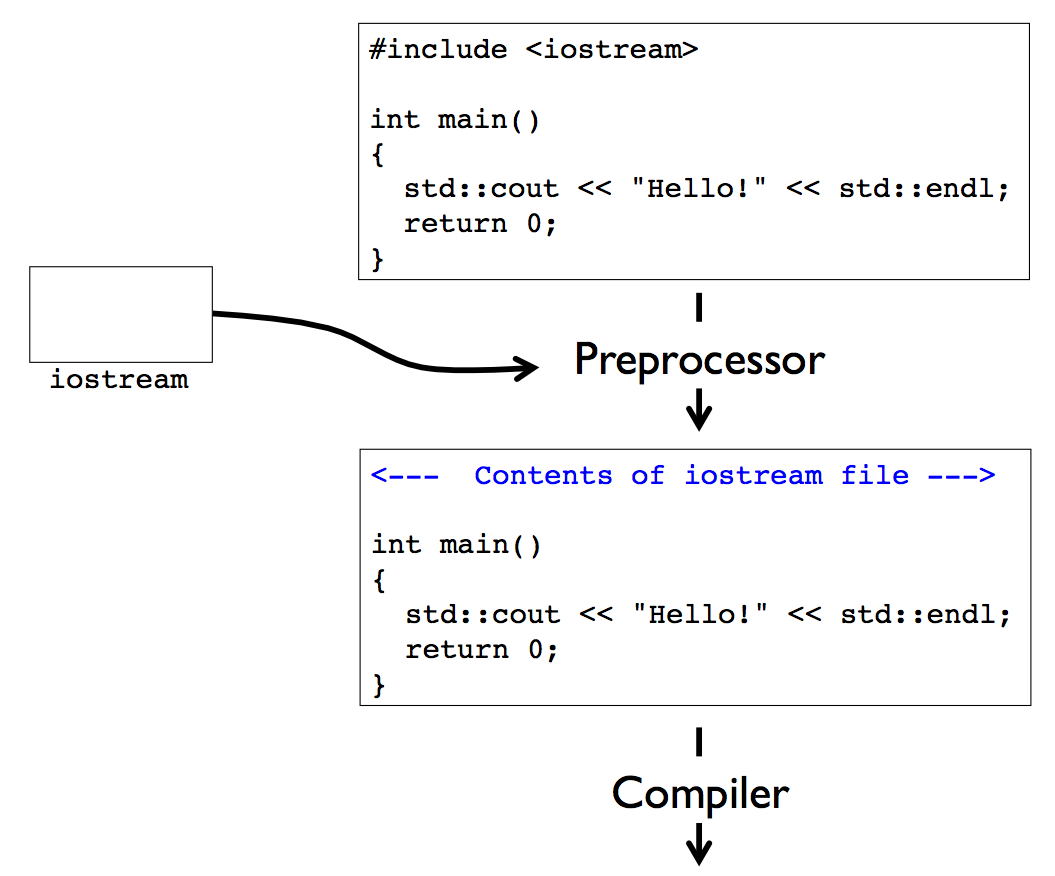
\includegraphics{fig/compilation.png}
\caption{fig}
\end{figure}

\subsubsection{Standard decomposition}
\begin{itemize}
\item
  Function (and type) \emph{declarations} go in header (\texttt{.hpp})
  files
\item
  Function \emph{definitions} go in source (\texttt{.cpp}) files
\item
  Source files that want to use the functions must \texttt{\#include}
  the header
\end{itemize}

\texttt{src/main6.cpp}:

\begin{cpp}
\begin{Highlighting}[]

\end{Highlighting}
\end{cpp}

\texttt{src/sum6.hpp}

\begin{cpp}
double sum(double a, double b);
\end{cpp}

\texttt{src/sum6.cpp}:

\begin{cpp}
#include "sum6.hpp"

double sum(double a, double b) {
  double c = a + b;
  return c;
}
\end{cpp}

Output:

\begin{verbatim}
$ g++ -Wall -Wextra -Wconversion main6.cpp sum6.cpp -o sum6
$ ./sum6
c = 5
\end{verbatim}

\subsubsection{\texorpdfstring{\texttt{\#include} syntax}{\#include syntax}}
\begin{itemize}
\item
  The \texttt{.hpp} file extension denotes a C++ header file
\item
  \texttt{\textless{}} \texttt{\textgreater{}} around the file name
  means that the preprocessor should search for an include file in a
  system dependent or default directory
\item
  These are typically include files that come with the compiler like
  \texttt{iostream}, \texttt{fstream}, \texttt{string}, etc.
\item
  Usually these files are somewhere in \texttt{/usr/include} with the
  GNU compilers on Linux
\item
  \texttt{"header.hpp"} means that the preprocessor should first search
  in the user directory, followed by a search in a system dependent or
  default directory if necessary
\end{itemize}

\subsubsection{\texorpdfstring{\texttt{\#define}}{\#define}}
\texttt{src/define1.cpp}:

\begin{cpp}
// define ni and nj to be 16

#define ni 16
#define nj 16

int main() {
  int a[ni][nj];

  for(int i = 0; i < ni; i++) {
    for(int j = 0; j < nj; j++) {
      a[i][j] = 1;
    }
  }

  return 0;
}
\end{cpp}

Pass the code through the preprocessor:

\begin{verbatim}
$ cpp -P define1.cpp
// define ni and nj to be 16

int main() {
  int a[16][16];

  for(int i = 0; i < 16; i++) {
    for(int j = 0; j < 16; j++) {
      a[i][j] = 1;
    }
  }

  return 0;
}
\end{verbatim}

\subsubsection{Macros}
\begin{itemize}
\item
  Real power of \texttt{\#define} is in setting up macros
\item
  Similar to functions but handled by the preprocessor
\end{itemize}

\subsubsection{\texorpdfstring{\texttt{\#define} macro}{\#define macro}}
\texttt{src/define2.cpp}

\begin{cpp}
#include <iostream>

#define sqr(n) (n)*(n)

int main() {
  int a = 2;

  int b = sqr(a);
  std::cout << "b = " << b << std::endl;

  return 0;
}
\end{cpp}

Output:

\begin{verbatim}
$ g++ -Wall -Wextra -Wconversion define2.cpp -o define2
$ ./define2
b = 4
\end{verbatim}

\subsubsection{Be careful}
\texttt{src/define3.cpp}:

\begin{cpp}
#include <iostream>

#define sqr(n) n*n

int main() {
  int a = 2;

  int b = sqr(a+3);
  std::cout << "b = " << b << std::endl;

  return 0;
}
\end{cpp}

Output:

\begin{verbatim}
$ g++ -Wall -Wextra -Wconversion define3.cpp -o define3
$ ./define3
b = 11
\end{verbatim}

\subsubsection{Predefined macros}
\texttt{src/define4.cpp}:

\begin{cpp}
\#include <iostream>

int main() {
  std::cout << "This line is in file " << __FILE__
            << ", line " << __LINE__ << std::endl;
  return 0;
}
\end{cpp}

Output:

\begin{verbatim}
$ g++ -Wall -Wextra -Wconversion define4.cpp -o define4
$ ./define4
This line is in file define4.cpp, line 5
\end{verbatim}

\subsubsection{Conditional compilation}
\texttt{src/conditional.cpp}:

\begin{cpp}
#include <iostream>

#define na 4

int main() {
  int a[na];

  a[0] = 2;
  for (int n = 1; n < na; n++) a[n] = a[n-1] + 1;

#ifdef DEBUG
  // Only kept by preprocessor if DEBUG defined
  for (int n = 0; n < na; n++) {
    std::cout << "a[" << n << "] = " << a[n] << std::endl;
  }
#endif

  return 0;
}
\end{cpp}

Output:

\begin{verbatim}
$ g++ -Wall -Wextra -Wconversion conditional.cpp -o conditional
$ ./conditional
$ g++ -Wall -Wextra -Wconversion conditional.cpp -o conditional -DDEBUG
$ ./conditional
a[0] = 2
a[1] = 3
a[2] = 4
a[3] = 5
\end{verbatim}

\subsubsection{Reading}
\begin{itemize}
\item
  \textbf{C++ Primer, Fifth Edition} by Lippman et al.
\item
  Chapter 6: Functions: Sections 6.1 - 6.3
\item
  Chapter 8: The IO Library
\item
  Chapter 17: Specialized Library Facilities: Section 17.5.1
\end{itemize}

\end{document}